
\setchapterimage[6cm]{intro/bucketsAndBalls/Basketball.png}
\setchapterpreamble[u]{\margintoc}
\chapter{Buckets and Balls\protect\footnotemark}
\labch{ch-bb}

\footnotetext{A basketball ball about to fall through the hoop. Author: \href{https://commons.wikimedia.org/wiki/File:2011-06-07_Basketball_in_hoop_still_shot.jpg}{Ildar Sagdejev / 2011 / GNU General Public License}.}
\footnotetext{This chapter is based on the article~\cite{bucketsAndBalls}.}

Linked Data is still largely unknown, or misunderstood and undervalued. Often, people find it simply too difficult. So I keep looking for new ways to make Linked Data more accessible. And with some success. In my training courses so far over 60\% of the participants had no IT background. I hope even to increase this percentage in the future.

What seems to be most challenging is writing SPARQL queries. The specification is written for IT people. There are some great courses and books but they also target people with some or more IT experience. If anything, that scares the rest and keeps SPARQL away from the masses.

I keep learning what is challenging. A recurring problem~--- and an unexpected one~--- is the concept of variable.

What is a variable in SPARQL? Just a placeholder. But how can you imagine a placeholder? It`s abstract. We have no way of grasping abstract things unless we associate them with something physical and concrete. It`s difficult to imagine time, but once we draw it in space it gets easier. We can`t picture furniture, but we have no problem with chair.

The other issue is how a SPARQL query looks. While working with SPARQL helps to understand how a knowledge graph works, a SPARQL query doesn`t look like one. It is like with symbols in mathematics. ``5~doesn`t look like five, while ||||| is five''. The problem with SPARQL is similar:

\begin{quote}
You want to query knowledge graph.\\
You want to learn new things.\\
But your query doesn`t look like knowledge graph.\\
It looks like lines of strings.\\
\end{quote}

So, how to handle together the problems with grasping variables and with the look of SPARQL?

My suggestion is to imagine every SPARQL query as a graph of linked buckets and balls.

Variables are placeholders but abstract. We need a physical container to fill with things. We need buckets. And nodes are like balls. So, think of running a query as filling buckets with balls.

A graph pattern then will look like this:

\begin{figure}[h!]
    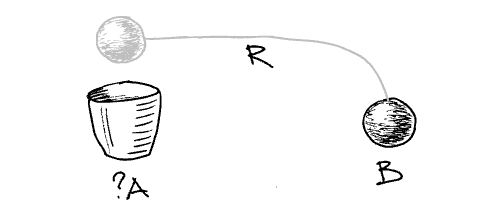
\includegraphics[width=0.6\linewidth]{./intro/bucketsAndBalls/graphPattern.PNG}
\end{figure}

A bucket \textbf{?A} should be filled with those balls which have a relation \textbf{R} to ball \textbf{B}.

But it looks nicer when we abbreviate it like this:

\begin{figure}[h]
    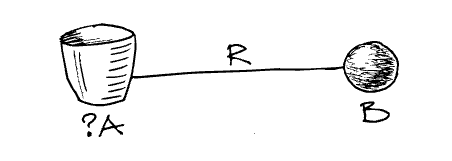
\includegraphics[width=0.6\linewidth]{./intro/bucketsAndBalls/graphPatternBucketsBalls.PNG}
\end{figure}

This is a graph pattern in Buckets`n`Balls notation. The direction of the relation R is not shown but it`s always from left to right.

The process of writing and running a SPARQL query would then go through the following steps:

\begin{enumerate}
    \item Select your buckets (in them you are going to gather the balls you want).
    \item Compose your conditions as a graph of buckets and balls.
    \item Run your query to fill your buckets with balls.
\end{enumerate}

Now let`s write a query to get all heads of government of the member states of the European Union, following these steps.

\begin{enumerate}
    \item We need two buckets, one for member states, one for heads of governments.
    \item The bucket for member state should be linked to the ball <<European union>> with relation <<member of>>; and it should be linked to the bucket for <<Head of Government>> with, well, the relation <<head of government>> which, respecting the direction should be thought of as <<has head of government>>.
\end{enumerate}

\newpage
Let`s make it more interesting and add another bucket for images. Here`s now the query in Buckets`n`Balls notation:

\begin{figure*}[h!]
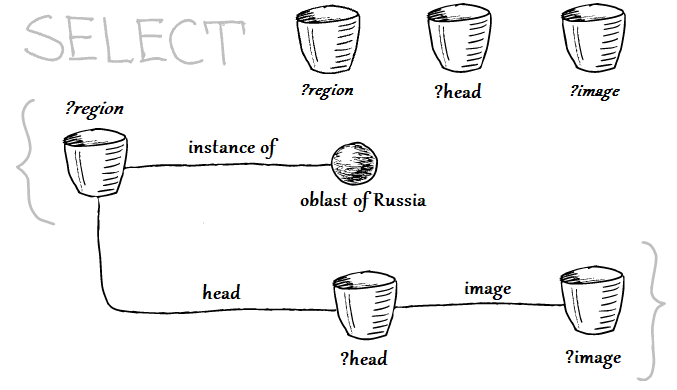
\includegraphics[width=0.55\linewidth]{./intro/bucketsAndBalls/select.PNG}
\end{figure*}

When we run the query, our buckets should, hopefully, look like this:

\begin{figure*}[h!]
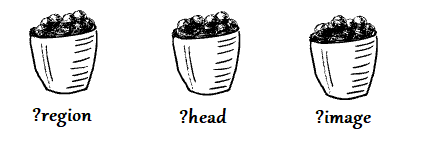
\includegraphics[width=0.55\linewidth]{./intro/bucketsAndBalls/query.PNG}
\end{figure*}

Now let`s go to Wikidata and write this query there.

Start by selecting the buckets to fill in.
